\documentclass{article}

\usepackage{pgfplots}
\pgfplotsset{compat=1.18}
\usepackage[a4paper,margin=0.1cm]{geometry}

% ================= CUSTOM COLOR + MARKER CYCLE =================
\pgfplotscreateplotcyclelist{crda_rda_cycle}{
% --- CRDA ---
{blue,   solid,  mark=*},
{red,    solid,  mark=square*},
{brown,  solid,  mark=triangle*},
% --- RDA ---
{green,  dashed, mark=*},
{gray,   dashed, mark=square*},
{purple, dashed, mark=triangle*},
}

\begin{document}

\begin{figure*}[t]
\centering

% ================= GLOBAL LEGEND =================
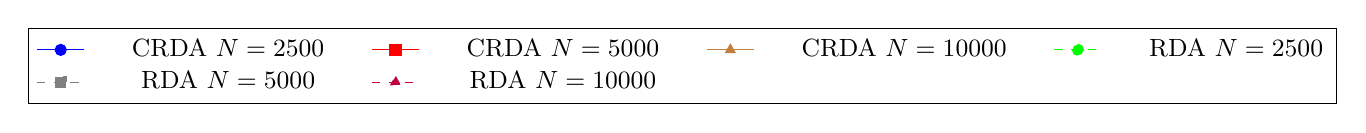
\begin{tikzpicture}
\begin{axis}[
    hide axis,
    xmin=0, xmax=1,
    ymin=0, ymax=1,
    legend columns=4,
    legend style={
        draw,
        at={(0.5,0)},
        anchor=north,
        column sep=1.5em,
        font=\small
    },
]
\addlegendimage{blue,   solid,  mark=*}
\addlegendentry{CRDA $N = 2500$}
\addlegendimage{red,    solid,  mark=square*}
\addlegendentry{CRDA $N = 5000$}
\addlegendimage{brown,  solid,  mark=triangle*}
\addlegendentry{CRDA $N = 10000$}

\addlegendimage{green,  dashed, mark=*}
\addlegendentry{RDA $N = 2500$}
\addlegendimage{gray,   dashed, mark=square*}
\addlegendentry{RDA $N = 5000$}
\addlegendimage{purple, dashed, mark=triangle*}
\addlegendentry{RDA $N = 10000$}
\end{axis}
\end{tikzpicture}
\vspace{0.5cm}

%%%%%%%%%%%%%%%%%%%%%%%%%%%%%%%%%%%%%%%%%%%%%%%%%%%%%%%%%%%%
% ===================== EPSILON = 0.05 ====================
%%%%%%%%%%%%%%%%%%%%%%%%%%%%%%%%%%%%%%%%%%%%%%%%%%%%%%%%%%%%

% --------- (1) k1 vs k2 ----------
\begin{minipage}[t]{0.33\textwidth}
\centering
\begin{tikzpicture}
\begin{axis}[
    width=\linewidth,
    height=4.5cm,
    xlabel={$k_2$},
    ylabel={$k_1$},
    title={$\epsilon = 0.05, k = 16$},
    grid=major,
    xmode=log,
    ymode=log,
    mark repeat=20,
    cycle list name=crda_rda_cycle,
]
\addplot table [x=k2,y=k1,col sep=comma] {estimates_k_16_eps5_N2500.csv};
\addplot table [x=k2,y=k1,col sep=comma] {estimates_k_16_eps5_N5000.csv};
\addplot table [x=k2,y=k1,col sep=comma] {estimates_k_16_eps5_N10000.csv};
\addplot table [x=k2,y=k1,col sep=comma] {estimates_data_eps5_N2500.csv};
\addplot table [x=k2,y=k1,col sep=comma] {estimates_data_eps5_N5000.csv};
\addplot table [x=k2,y=k1,col sep=comma] {estimates_data_eps5_N10000.csv};
\end{axis}
\end{tikzpicture}
\end{minipage}%
\hfill

% --------- (2) Data Duplication ----------
\begin{minipage}[t]{0.33\textwidth}
\centering
\begin{tikzpicture}
\begin{axis}[
    width=\linewidth,
    height=4.5cm,
    xlabel={$k_2$},
    ylabel={$Data\ Duplication$},
    title={$\epsilon = 0.05, k = 16$},
    grid=major,
    xmode=log,
    ymode=log,
    mark repeat=20,
    cycle list name=crda_rda_cycle,
]
\addplot table [x=k2,y=data_duplication,col sep=comma] {estimates_k_16_eps5_N2500.csv};
\addplot table [x=k2,y=data_duplication,col sep=comma] {estimates_k_16_eps5_N5000.csv};
\addplot table [x=k2,y=data_duplication,col sep=comma] {estimates_k_16_eps5_N10000.csv};
\addplot table [x=k2,y=data_duplication,col sep=comma] {estimates_data_eps5_N2500.csv};
\addplot table [x=k2,y=data_duplication,col sep=comma] {estimates_data_eps5_N5000.csv};
\addplot table [x=k2,y=data_duplication,col sep=comma] {estimates_data_eps5_N10000.csv};
\end{axis}
\end{tikzpicture}
\end{minipage}%
\hfill

% --------- (3) Store Complexity ----------
\begin{minipage}[t]{0.33\textwidth}
\centering
\begin{tikzpicture}
\begin{axis}[
    width=\linewidth,
    height=4.5cm,
    xlabel={$k_2$},
    ylabel={$Store\ Complexity$},
    title={$\epsilon = 0.05, k = 16$},
    grid=major,
    xmode=log,
    ymode=log,
    mark repeat=20,
    cycle list name=crda_rda_cycle,
]
\addplot table [x=k2,y=store_complexity,col sep=comma] {estimates_k_16_eps5_N2500.csv};
\addplot table [x=k2,y=store_complexity,col sep=comma] {estimates_k_16_eps5_N5000.csv};
\addplot table [x=k2,y=store_complexity,col sep=comma] {estimates_k_16_eps5_N10000.csv};
\addplot table [x=k2,y=store_complexity,col sep=comma] {estimates_data_eps5_N2500.csv};
\addplot table [x=k2,y=store_complexity,col sep=comma] {estimates_data_eps5_N5000.csv};
\addplot table [x=k2,y=store_complexity,col sep=comma] {estimates_data_eps5_N10000.csv};
\end{axis}
\end{tikzpicture}
\end{minipage}

\vspace{0.5cm}

%%%%%%%%%%%%%%%%%%%%%%%%%%%%%%%%%%%%%%%%%%%%%%%%%%%%%%%%%%%%
% ===================== EPSILON = 0.10 ====================
%%%%%%%%%%%%%%%%%%%%%%%%%%%%%%%%%%%%%%%%%%%%%%%%%%%%%%%%%%%%

% --------- (4) k1 vs k2 ----------
\begin{minipage}[t]{0.33\textwidth}
\centering
\begin{tikzpicture}
\begin{axis}[
    width=\linewidth,
    height=4.5cm,
    xlabel={$k_2$},
    ylabel={$k_1$},
    title={$\epsilon = 0.1, k = 16$},
    grid=major,
    xmode=log,
    ymode=log,
    mark repeat=20,
    cycle list name=crda_rda_cycle,
]
\addplot table [x=k2,y=k1,col sep=comma] {estimates_k_16_eps10_N2500.csv};
\addplot table [x=k2,y=k1,col sep=comma] {estimates_k_16_eps10_N5000.csv};
\addplot table [x=k2,y=k1,col sep=comma] {estimates_k_16_eps10_N10000.csv};
\addplot table [x=k2,y=k1,col sep=comma] {estimates_data_eps10_N2500.csv};
\addplot table [x=k2,y=k1,col sep=comma] {estimates_data_eps10_N5000.csv};
\addplot table [x=k2,y=k1,col sep=comma] {estimates_data_eps10_N10000.csv};
\end{axis}
\end{tikzpicture}
\end{minipage}%
\hfill

% --------- (5) Data Duplication ----------
\begin{minipage}[t]{0.33\textwidth}
\centering
\begin{tikzpicture}
\begin{axis}[
    width=\linewidth,
    height=4.5cm,
    xlabel={$k_2$},
    ylabel={$Data\ Duplication$},
    title={$\epsilon = 0.1, k = 16$},
    grid=major,
    xmode=log,
    ymode=log,
    mark repeat=20,
    cycle list name=crda_rda_cycle,
]
\addplot table [x=k2,y=data_duplication,col sep=comma] {estimates_k_16_eps10_N2500.csv};
\addplot table [x=k2,y=data_duplication,col sep=comma] {estimates_k_16_eps10_N5000.csv};
\addplot table [x=k2,y=data_duplication,col sep=comma] {estimates_k_16_eps10_N10000.csv};
\addplot table [x=k2,y=data_duplication,col sep=comma] {estimates_data_eps10_N2500.csv};
\addplot table [x=k2,y=data_duplication,col sep=comma] {estimates_data_eps10_N5000.csv};
\addplot table [x=k2,y=data_duplication,col sep=comma] {estimates_data_eps10_N10000.csv};
\end{axis}
\end{tikzpicture}
\end{minipage}%
\hfill

% --------- (6) Store Complexity ----------
\begin{minipage}[t]{0.33\textwidth}
\centering
\begin{tikzpicture}
\begin{axis}[
    width=\linewidth,
    height=4.5cm,
    xlabel={$k_2$},
    ylabel={$Store\ Complexity$},
    title={$\epsilon = 0.1, k = 16$},
    grid=major,
    xmode=log,
    ymode=log,
    mark repeat=20,
    cycle list name=crda_rda_cycle,
]
\addplot table [x=k2,y=store_complexity,col sep=comma] {estimates_k_16_eps10_N2500.csv};
\addplot table [x=k2,y=store_complexity,col sep=comma] {estimates_k_16_eps10_N5000.csv};
\addplot table [x=k2,y=store_complexity,col sep=comma] {estimates_k_16_eps10_N10000.csv};
\addplot table [x=k2,y=store_complexity,col sep=comma] {estimates_data_eps10_N2500.csv};
\addplot table [x=k2,y=store_complexity,col sep=comma] {estimates_data_eps10_N5000.csv};
\addplot table [x=k2,y=store_complexity,col sep=comma] {estimates_data_eps10_N10000.csv};
\end{axis}
\end{tikzpicture}
\end{minipage}

\caption{(left) $k_1$ vs. $k_2$, (middle) data duplication vs. $k_2$, and (right) storage complexity vs. $k_2$, comparing RobustCDA and RDA across $N \in \{2500, 5000, 10000\}$.}
\end{figure*}

\end{document}